\documentclass[A4paper]{gdv/gdv}
\usepackage{epic}
\usepackage{eepic}
\usepackage{amssymb,amsmath}
\usepackage{version}
\usepackage{url}
\usepackage[T1]{fontenc}
% \usepackage[applemac]{inputenc} % MacOSX
\usepackage[utf8]{inputenc} % Linux
\usepackage[margin=10pt,labelfont=bf]{caption}        
\newcommand{\til}{\raise.17ex\hbox{$\scriptstyle\sim$}}
\newcommand{\todo}[1]{\textbf{Todo:\ #1}}
\newcommand{\note}{\textit{Note:}\ }
\newcommand{\teilaufgabe}[1]{\textbf{#1.}}
\begin{document}
\begin{gdvSheet}
% hier müssen whitespaces hin!
  
\kopf{Philipp Koegel, Bastian Mattes, Jan Doerntlein}{07.01.2015}{GraPro: Graphics Project}{5}
\newcommand{\file}[1]{\texttt{#1}}
\newcommand{\code}[1]{\texttt{#1}}
%########################################################################################

\aufgabe{1}{4}{OpenGL Framework.} 
The following assignments are based on a OpenGL 4.4 engine that is written from scratch. 

\teilaufgabe{1. Basic Setup (1 Punkte)} Wrapper classes for easy use of shaders, materials, debugging etc. \\
\teilaufgabe{2. Object loading (1 Punkte)} Use Assimp to load Wavefront obj/mtl files. \\
\teilaufgabe{3. Texturing (1 Punkte)} Implement Blinn/Phong shading and load a scene textured. \\
\teilaufgabe{4. GUI (1 Punkte)} Integrate a GUI library. \\

\begin{figure}[h]
\centering
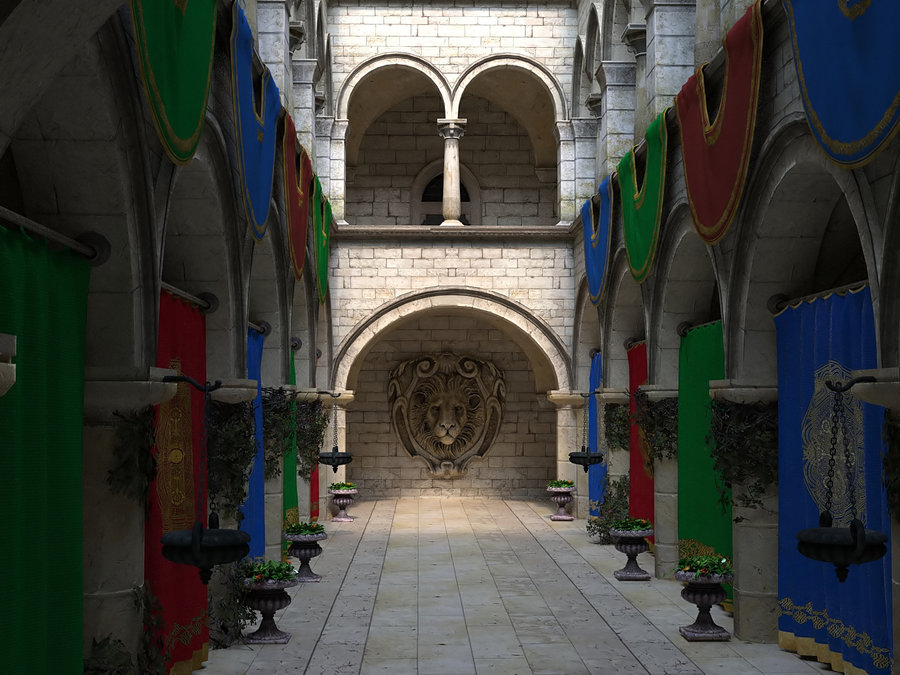
\includegraphics[width=300px]{img/sponza.jpg}
\caption{Possible result of assignment 1.}
\end{figure}

\aufgabe{2}{12}{Voxel Cone Tracing.} 
The indirect illumination algorithms implemented in the previous assignments are computationally expensive. Using accelerating data structures like BVHs or kd-trees results in greats speed ups but still the time to render an image is far from real time. While this is almost impossible to accomplish with CPU rendering there are still ways to gain some more speed without a perceivable loss in quality. \\
\\
The algorithm of Crassin, Cyril, et al. encapsulates a number of rays with approximately the same direction in a ray cluster. This cluster is represented as a cone. In a preprocessing step the scene is rendered from the light sources and the radiance and light direction is saved in an octree. The visibility and the energy of the cone can then be estimated very fast by testing against the voxels of the octree. If the result is not relevant for the upcoming computations all rays in one cluster can be discarded.

\teilaufgabe{1. Octree (4 Punkte)} Render from light sources and bake incoming radiance and light direction into the octree. \\
\teilaufgabe{2. Filtering (4 Punkte)} Filter irradiance values and light directions inside the octree. \\
\teilaufgabe{3. Rendering (4 Punkte)} Render from camera and sample BxDF using voxel based cone tracing. \\

\begin{figure}[h]
\centering
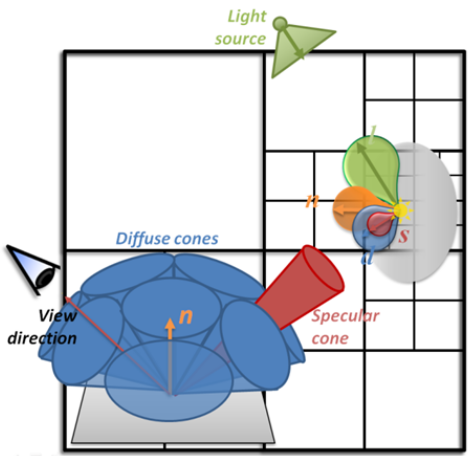
\includegraphics[width=150px]{img/voxel.png}
\caption{Voxel Cone Tracing.}
\end{figure}
  
\aufgabe{3}{4}{Extensions for assignment 2.} 
To create a more realistic look of the voxel cone tracing algorithm it is extended with an ambient occlusion (not in screen space) technique here. Furthermore the meshes should support emissive material.

\teilaufgabe{1. Ambient Occlusion (2 Punkte)} Ambient Occlusion implementation. \\
\teilaufgabe{2. Area Lights (2 Punkte)} Emissive Material. \\

\begin{figure}[h]
\centering
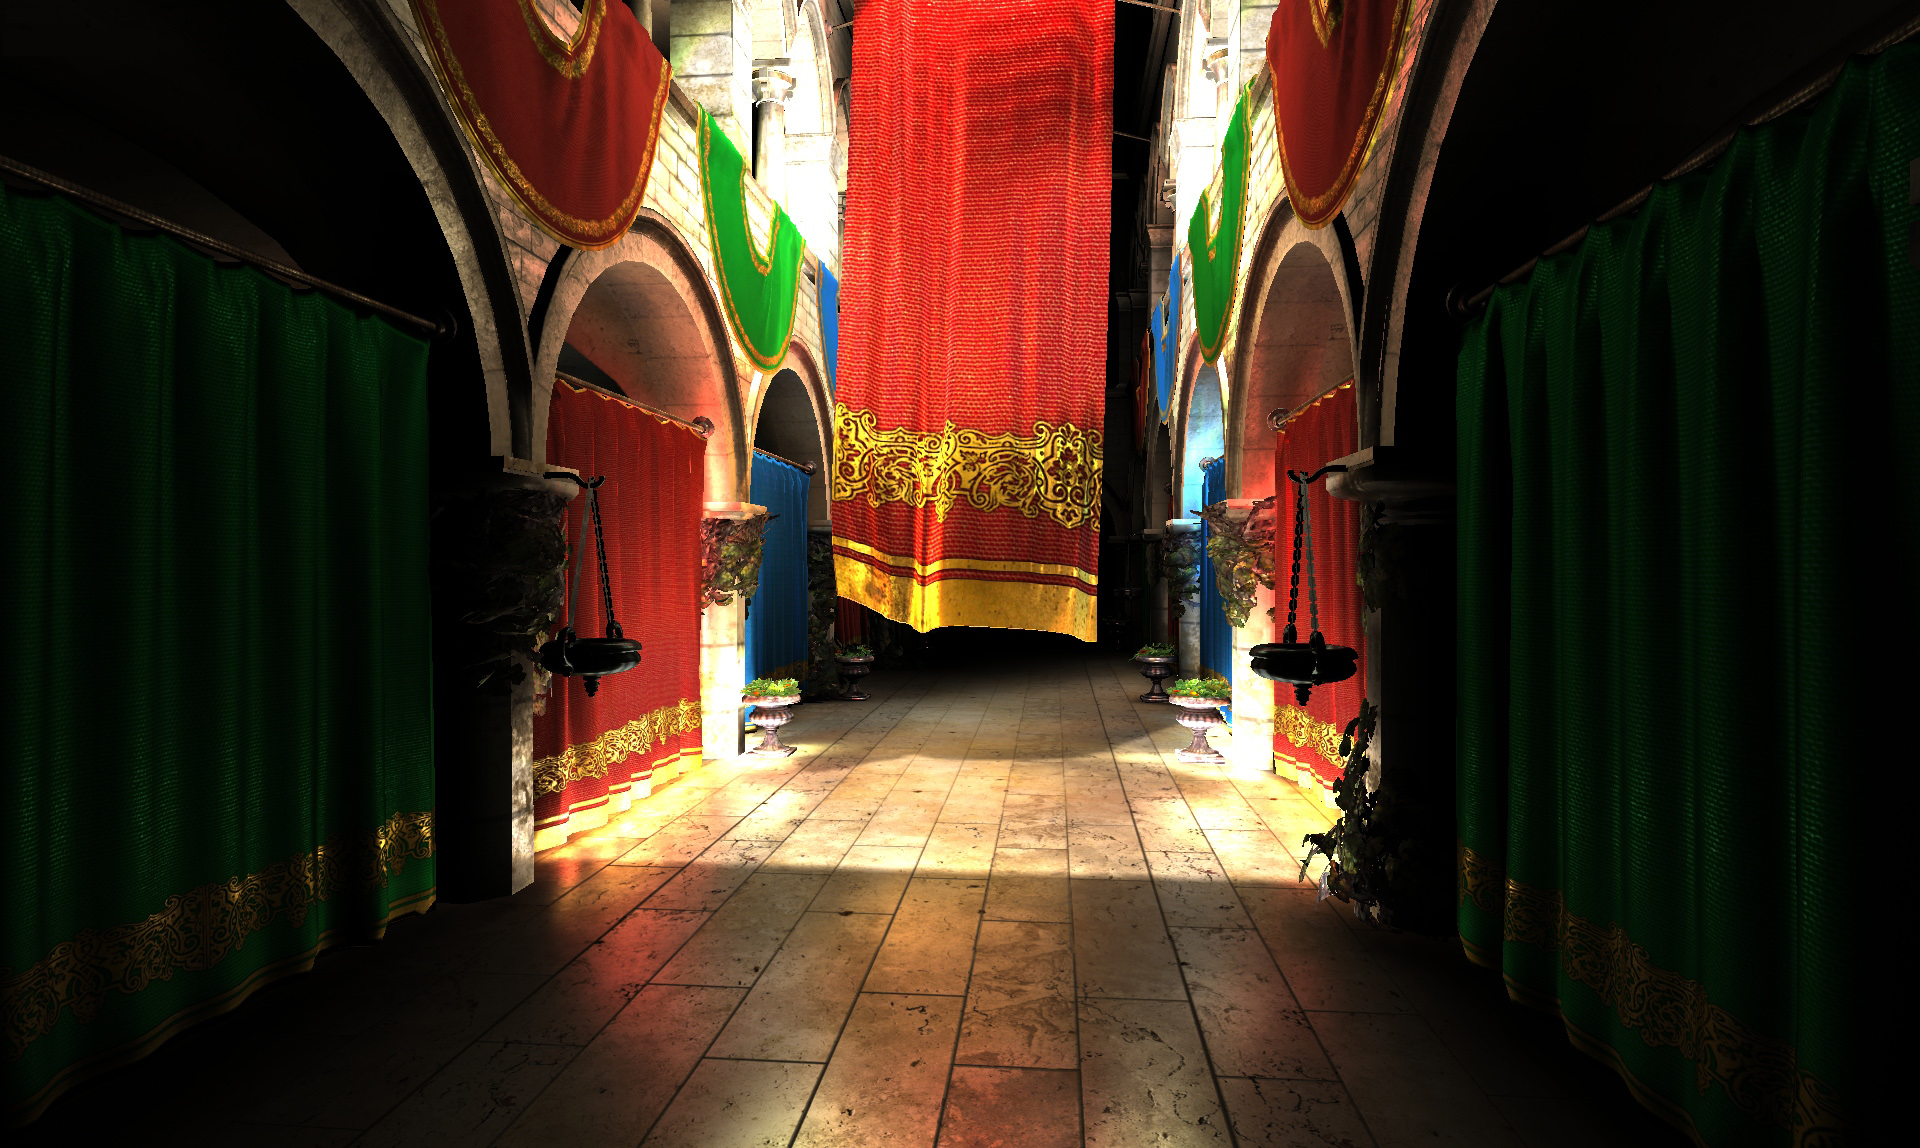
\includegraphics[width=450px]{img/sponza-voxelcone.jpg}
\caption{Possible result after assignment 3.}
\end{figure}

% \aufgabe{4}{4}{Smoke Rendering Using Compensated Ray Marching.}
% In this assignment the Aurora framework is extended to support smoke rendering. Due to the complex parts above this exercise is more like a bonus. The algorithm of Zhou, Kun, et al. is used in real time applications (on GPU) and promises fast results on the CPU as well. Several acceleration strategies and approximations are used in this technique. \\
% \\
% The algorithm looks very sophisticated so maybe we cut it down to reduce the workload (and maybe the speed) while still implementing a simpler method to render smoke.
% 
% \teilaufgabe{1. Density field approximation (1 Punkt)} \\
% \teilaufgabe{2. Resiudal field compression (1 Punkt)} \\
% \teilaufgabe{3. Light scattering (1 Punkt)} \\
% \teilaufgabe{4. Compensated ray marching algorithm (1 Punkt)} \\
% 
% \begin{figure}[h]
% \centering
% 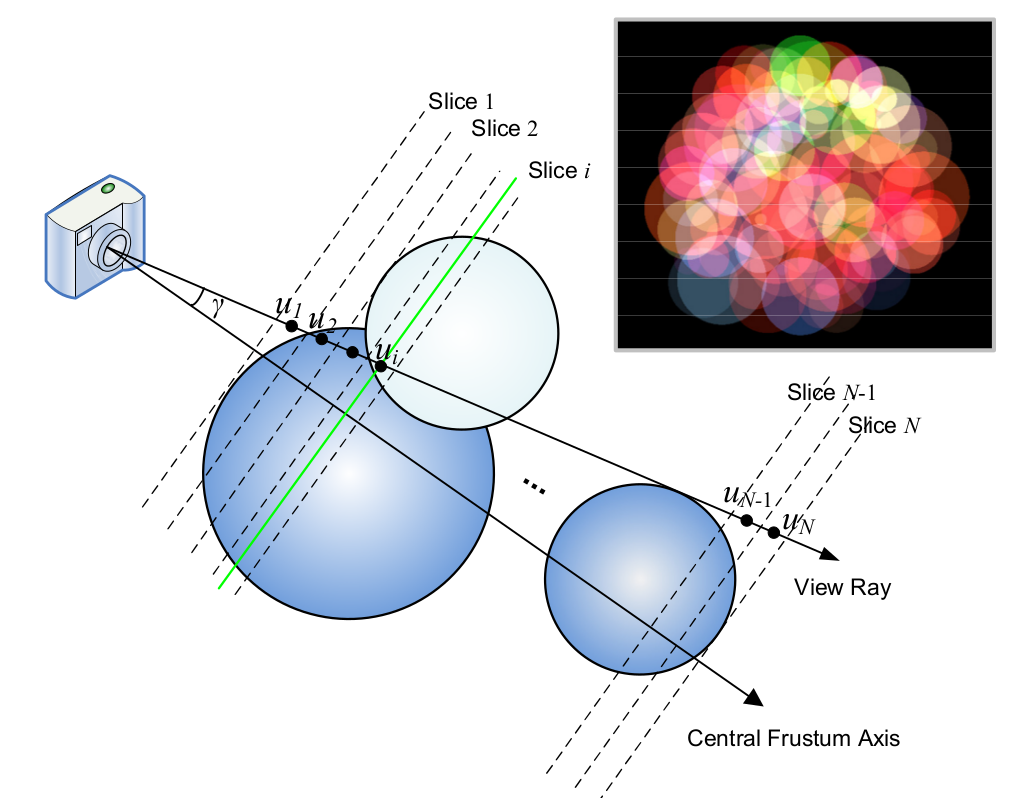
\includegraphics[width=200px]{img/smoke.png}
% \caption{View pass in ray marching.}
% \end{figure}
% 
Sources:
\begin{enumerate}
\item Crassin, Cyril, et al. ``Interactive indirect illumination using voxel cone tracing.'' Computer Graphics Forum. Vol. 30. No. 7. Blackwell Publishing Ltd, 2011.
\item Zhou, Kun, et al. ``Real-time smoke rendering using compensated ray marching.'' ACM Transactions on Graphics (TOG). Vol. 27. No. 3. ACM, 2008.
\end{enumerate}

\vfill
% \pagebreak
% \bibliographystyle{plain}
% \bibliography{lit}
% \vfill\hfill Happy Hacking! :) \hfill\ %\vfill
\end{gdvSheet}
\end{document}
